\StartPlate{V25}{A single transvection repairs an isotropic defect}{The repair is explicit, and the previously correct line stays fixed.}
\begin{center}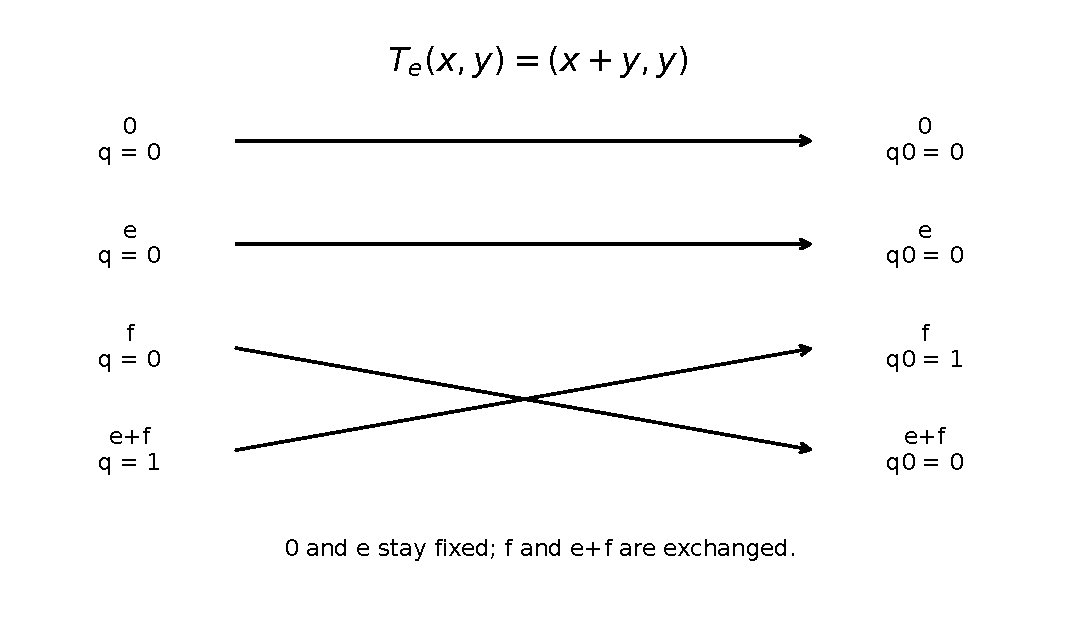
\includegraphics[width=\linewidth]{figures/V25.pdf}\end{center}
Take $q(x,y)=xy$ and $q_0(x,y)=xy+y$. Their discrepancy is $B(e,-)$, with $e=(1,0)$ and $q(e)=0$. The transvection is
\[
T_e(x,y)=(x+y,y),\qquad q_0(T_e v)=q(v).
\]
The arrows show its action on every vector. Zero and $e$ remain fixed. The vectors $f$ and $e+f$ exchange places. Each arrow therefore lands on the same quadratic value shown at its source.

The original identity map did not work: $q(f)=0$ while $q_0(f)=1$. Matching Arf invariants guarantees a correction here, not the validity of an unchanged map. More generally, a defect vanishing on a subspace $U$ gives a defect vector in $U^\perp$, so the transvection fixes $U$ pointwise.

The correction fixes quotient vectors, not automatically independently fixed lifts above them. Its use in an arithmetic diagram requires permission to change the embedding and a separate check of the relevant section and phase data.
\vfill\PlateSource{Exact four-vector correction}{Part III, Section 28.1--28.3}{71}
